\documentclass[10pt]{article}

\usepackage{graphicx}
\usepackage{caption}
\usepackage{subcaption}
\usepackage[utf8]{inputenc}   
\usepackage[T1]{fontenc}

\title{Utilisation écrans intéractifs Speechi}
\author{Nicolas Barrier}

\begin{document}
\maketitle
\tableofcontents
\section{Precautions d'usage et bonnes pratiques}

Avant de commencer, voici quelques précautions d'usage et bonnes pratiques avant l'utilisation des écrans.

\begin{itemize}
\item Manipuler avec précaution les pieds lors des déplacements des écrans.
\item Procéder avec précaution lors de l'ajustement en hauteur (via les poignées).
\item Eteindre complètement les écrans après utilisation (bouton situé sous l'écran au niveau de l'alimentation)
\item Replier les antennes du PC (côté de l'écran)
\end{itemize}

\section{Matériel}

Chaque écran est livré avec:

\begin{itemize}
\item 1 cable HDMI
\item 1 cable USB
\item 1 cordon d’alimentation
\item 1 télécommande
\item 2 stylets
\item 1 clavier sans fil
\end{itemize}

\textbf{Merci de ne pas emporter ce matériel avec vous!}\\ 

\emph{Note: en salle ScenarioLab, utiliser le clavier qui correspond à l'écran utilisé (cf. étiquettes).}

\section{Double système}

Les écrans sont équipés de deux systèmes indépendants:

\begin{itemize}
\item 1 système Android  (Figure \ref{fig:sys-andro})
\item 1 système Windows (Figure \ref{fig:sys-win})
\end{itemize}

\begin{figure}[h!]
	\centering
  	\begin{subfigure}[b]{0.4\textwidth}
		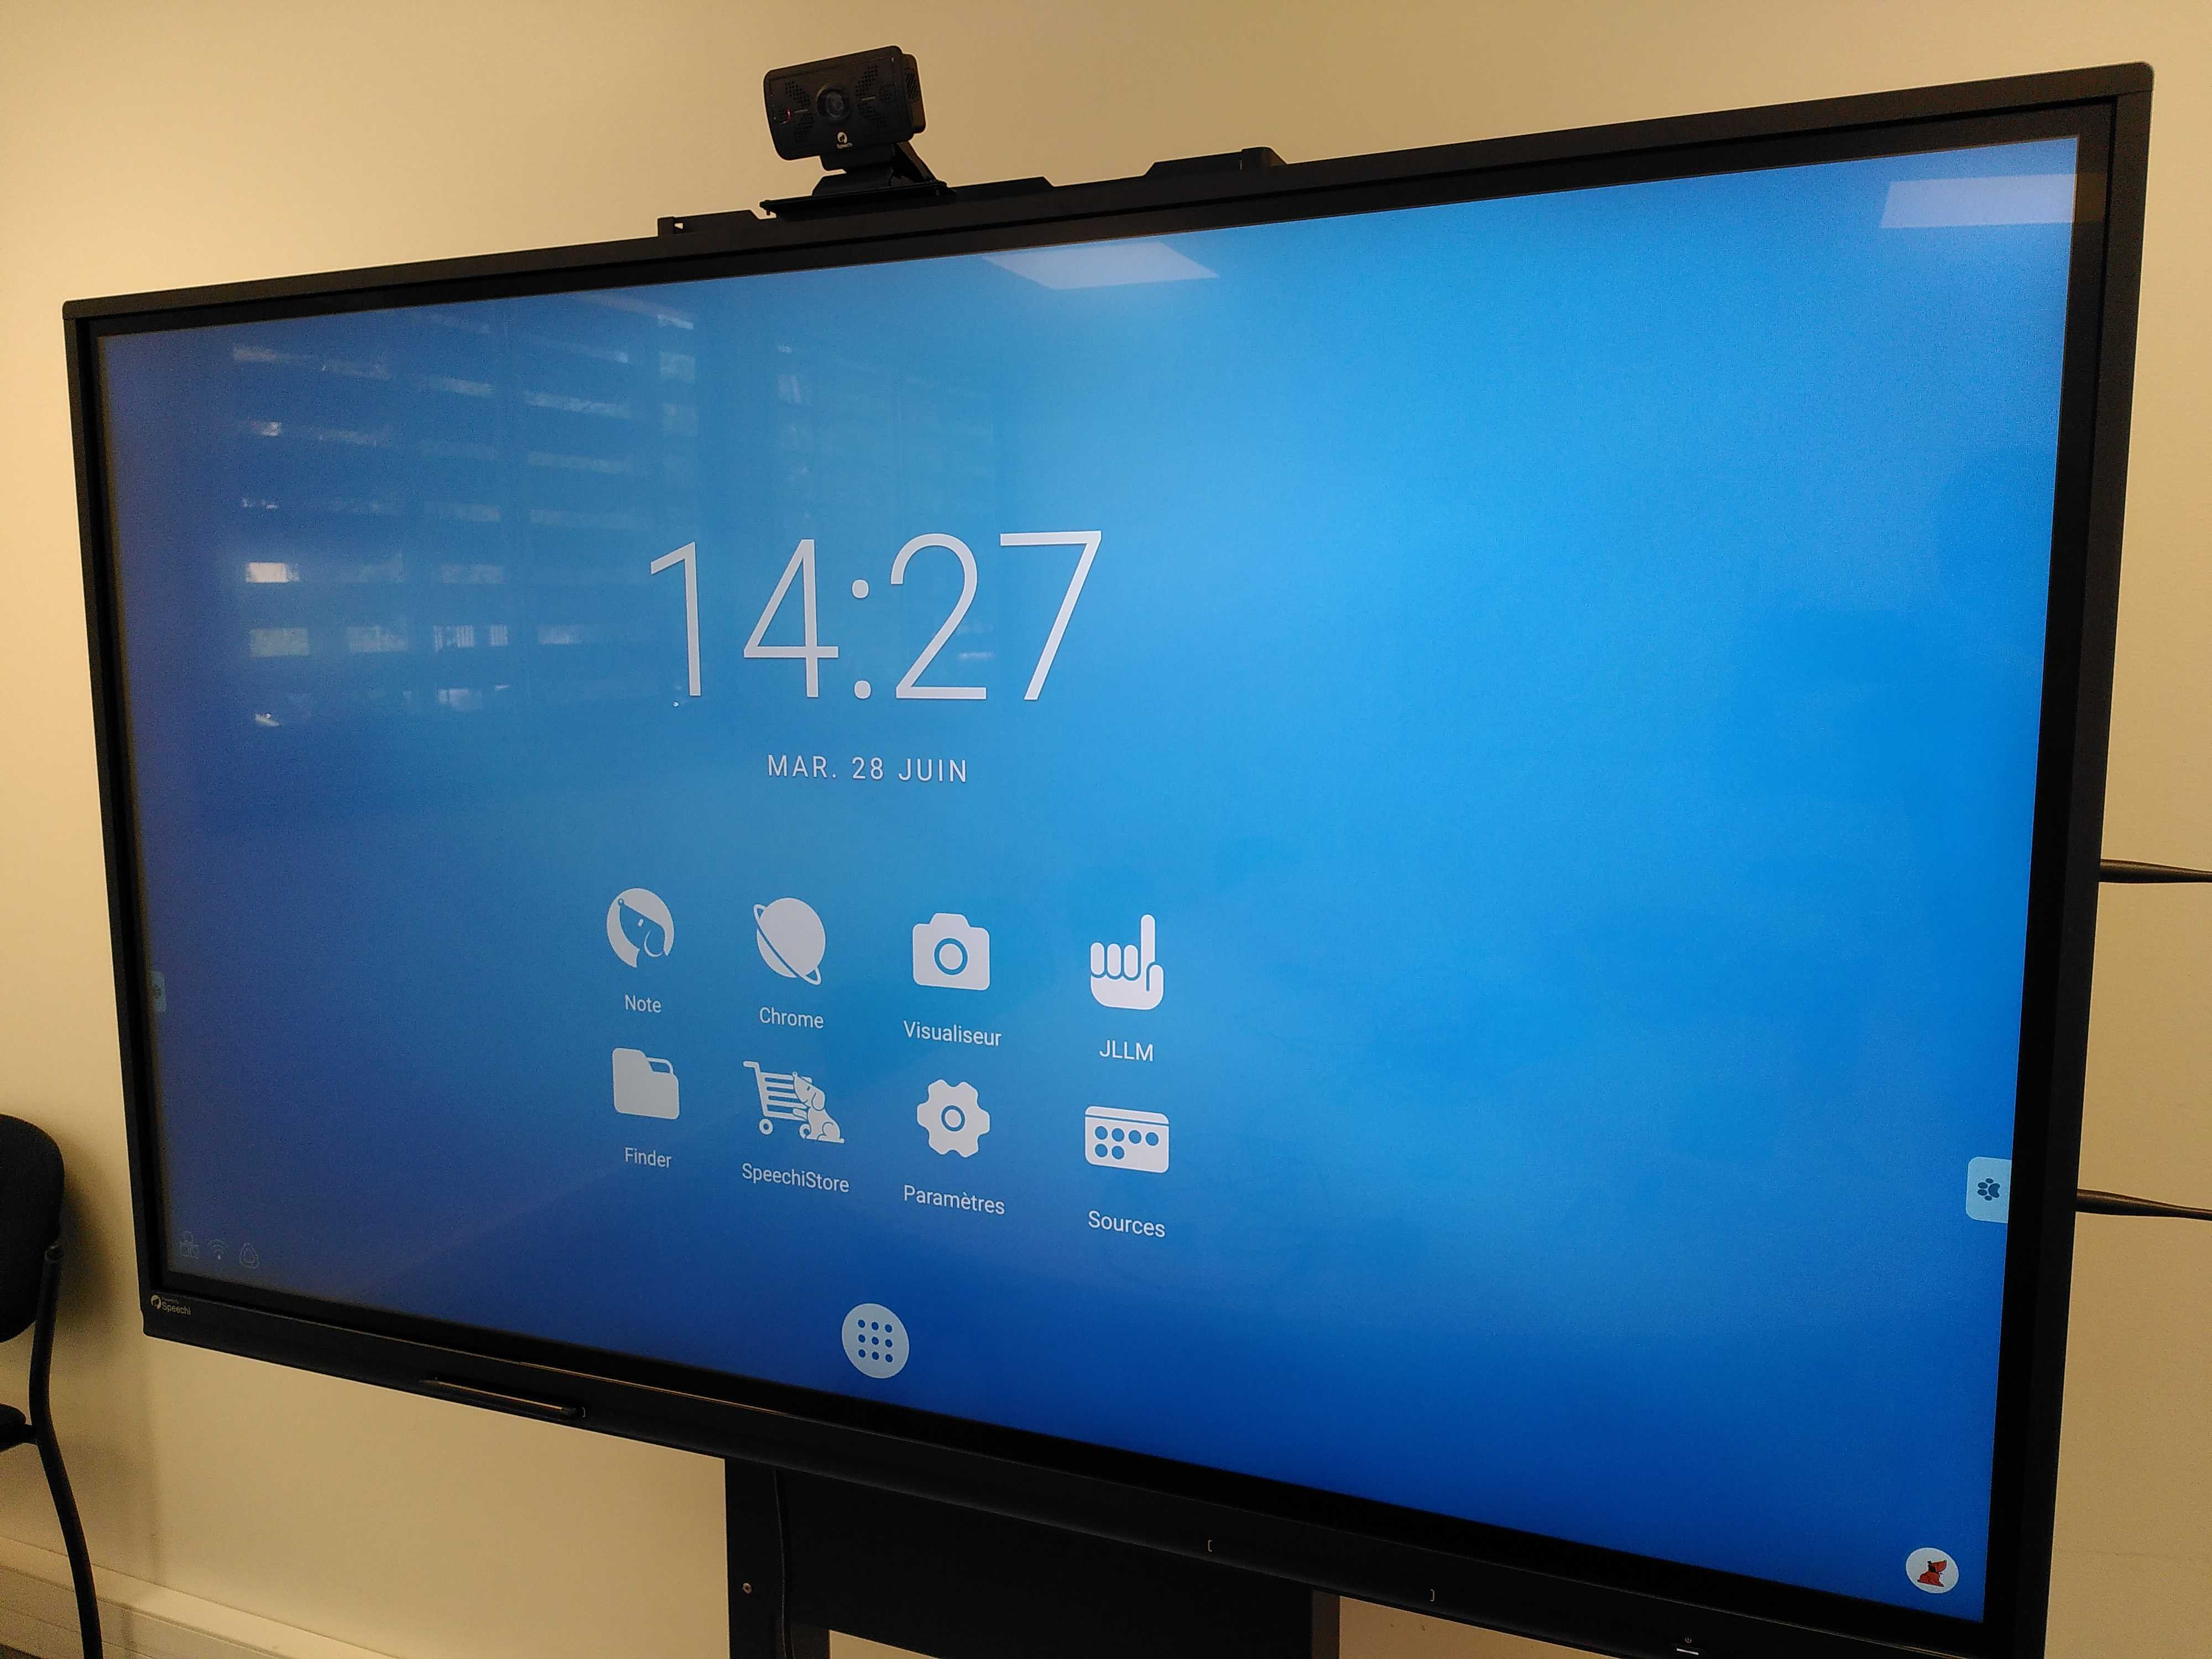
\includegraphics[width=\textwidth]{IMG_20220628_142750.jpg}
		\caption{Systeme Android}
		\label{fig:sys-andro}
	\end{subfigure}
	\hfill
 	\begin{subfigure}[b]{0.4\textwidth}
		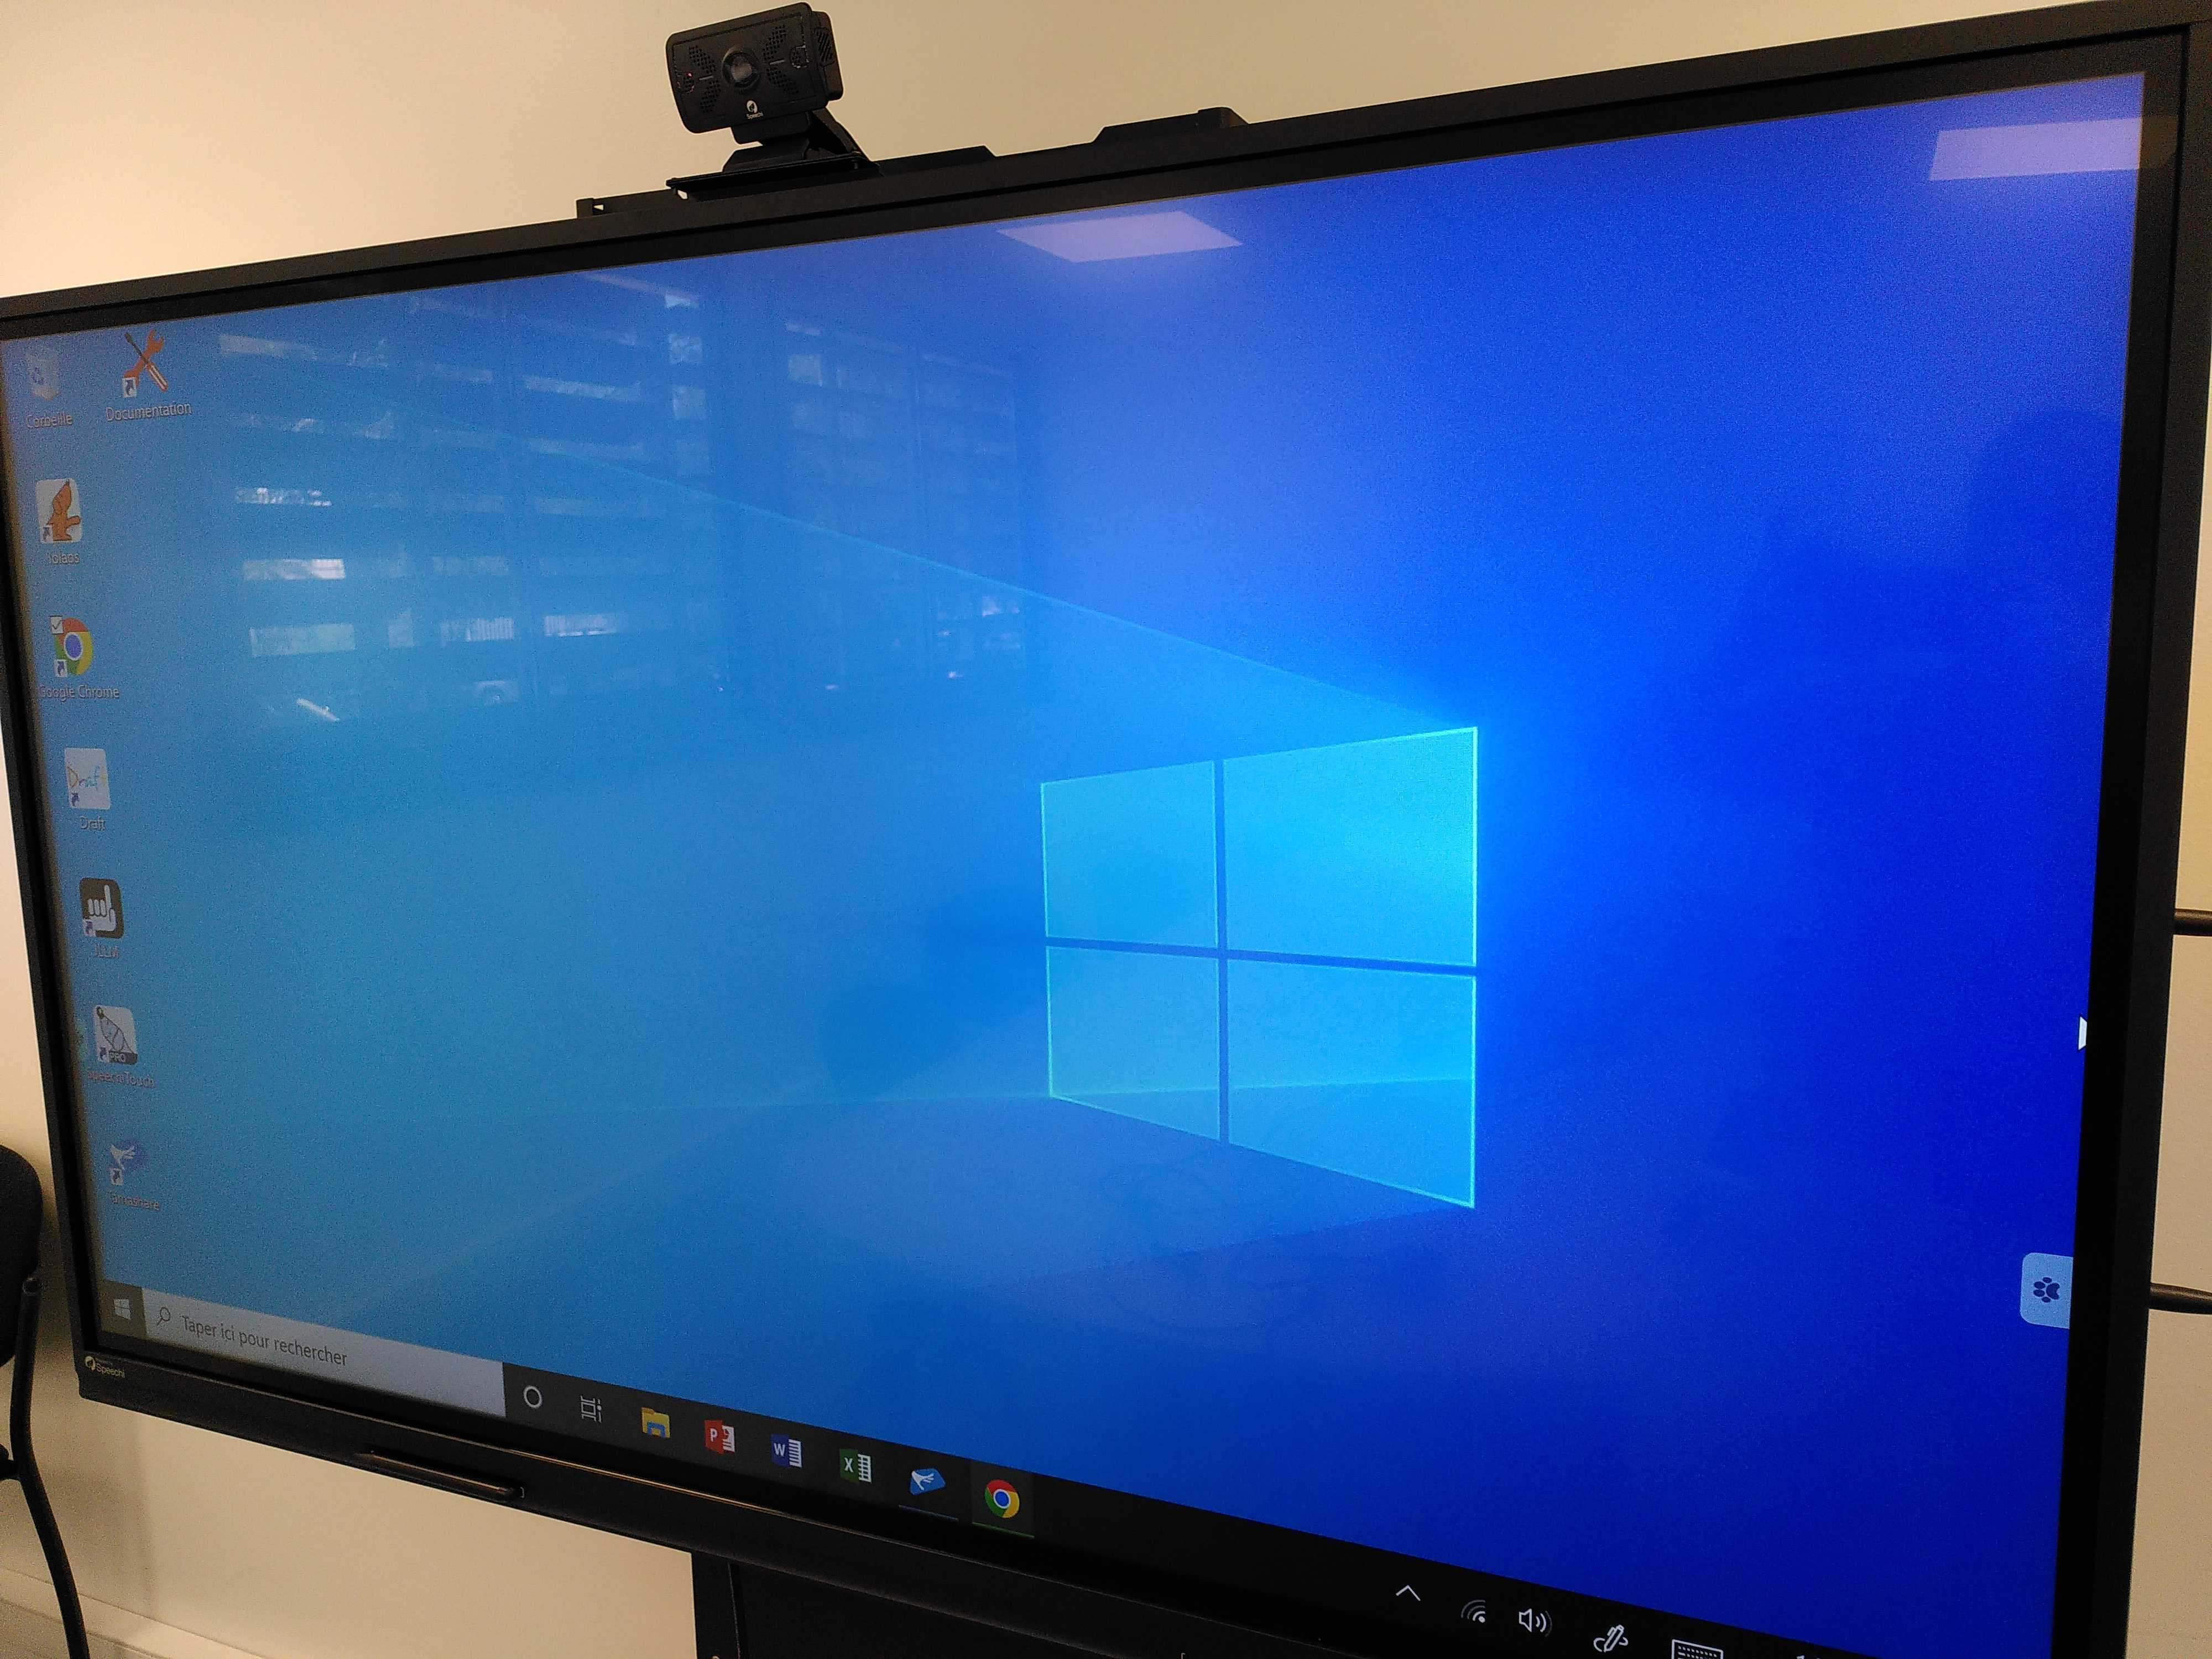
\includegraphics[width=\textwidth]{IMG_20220628_143733.jpg}
		\caption{Systeme Windows}
		\label{fig:sys-win}
	\end{subfigure}
	\caption{Double système}
\end{figure}

Pour changer de systeme, cliquer sur le symbole "Patte" sur un des côtés de l'écran (Figure \ref{fig:symb-patte}), puis sur le symbole "Source" (carré contenant 6 cercles, cf. Figure \ref{fig:symb-source}).\\

Pour utiliser le système Windows, choisir "PC", pour choisir le système Android, cliquer sur "Android" (Figure \ref{fig:sources}).\\

\emph{Note: cette manipulation permet aussi de changer la source, par exemple si on branche un PC sur port HDMI ou autre}.\\

\begin{figure}[h!]
	\centering
  	\begin{subfigure}[b]{0.4\textwidth}
		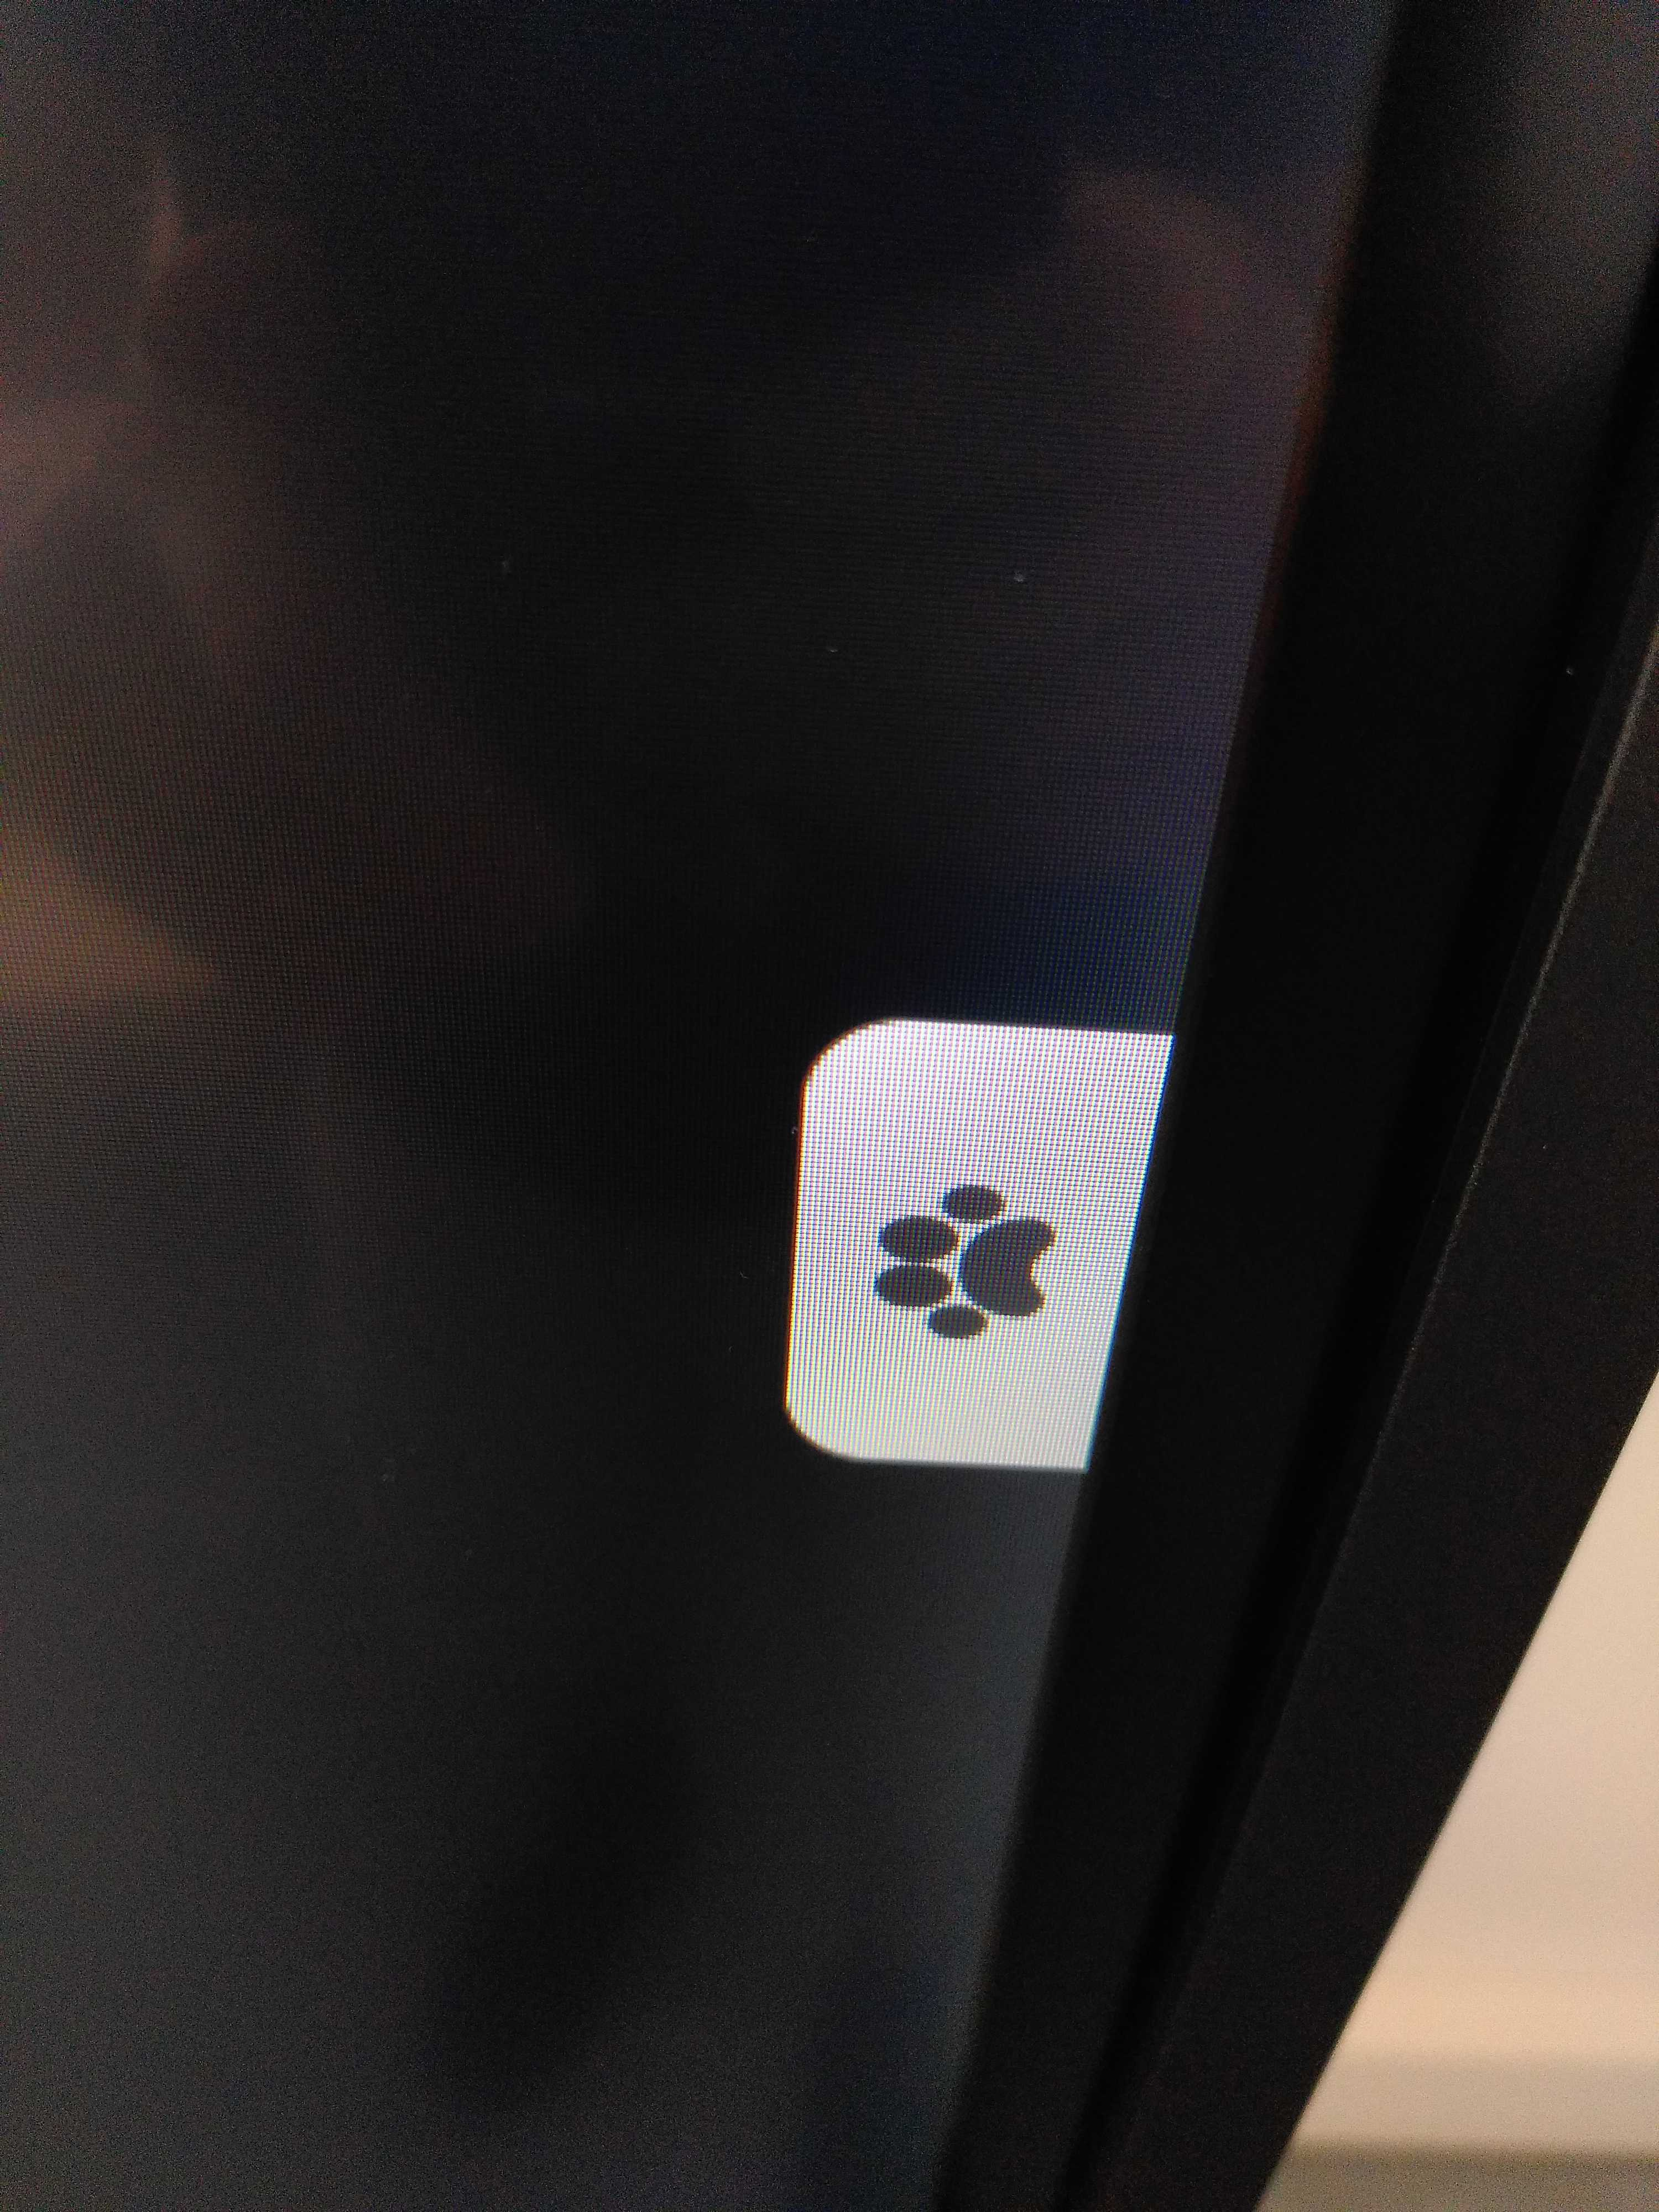
\includegraphics[width=\textwidth]{IMG_20220628_165539.jpg}
		\caption{Symbole "Patte"}
		\label{fig:symb-patte}
	\end{subfigure}
	\hfill
 	\begin{subfigure}[b]{0.4\textwidth}
		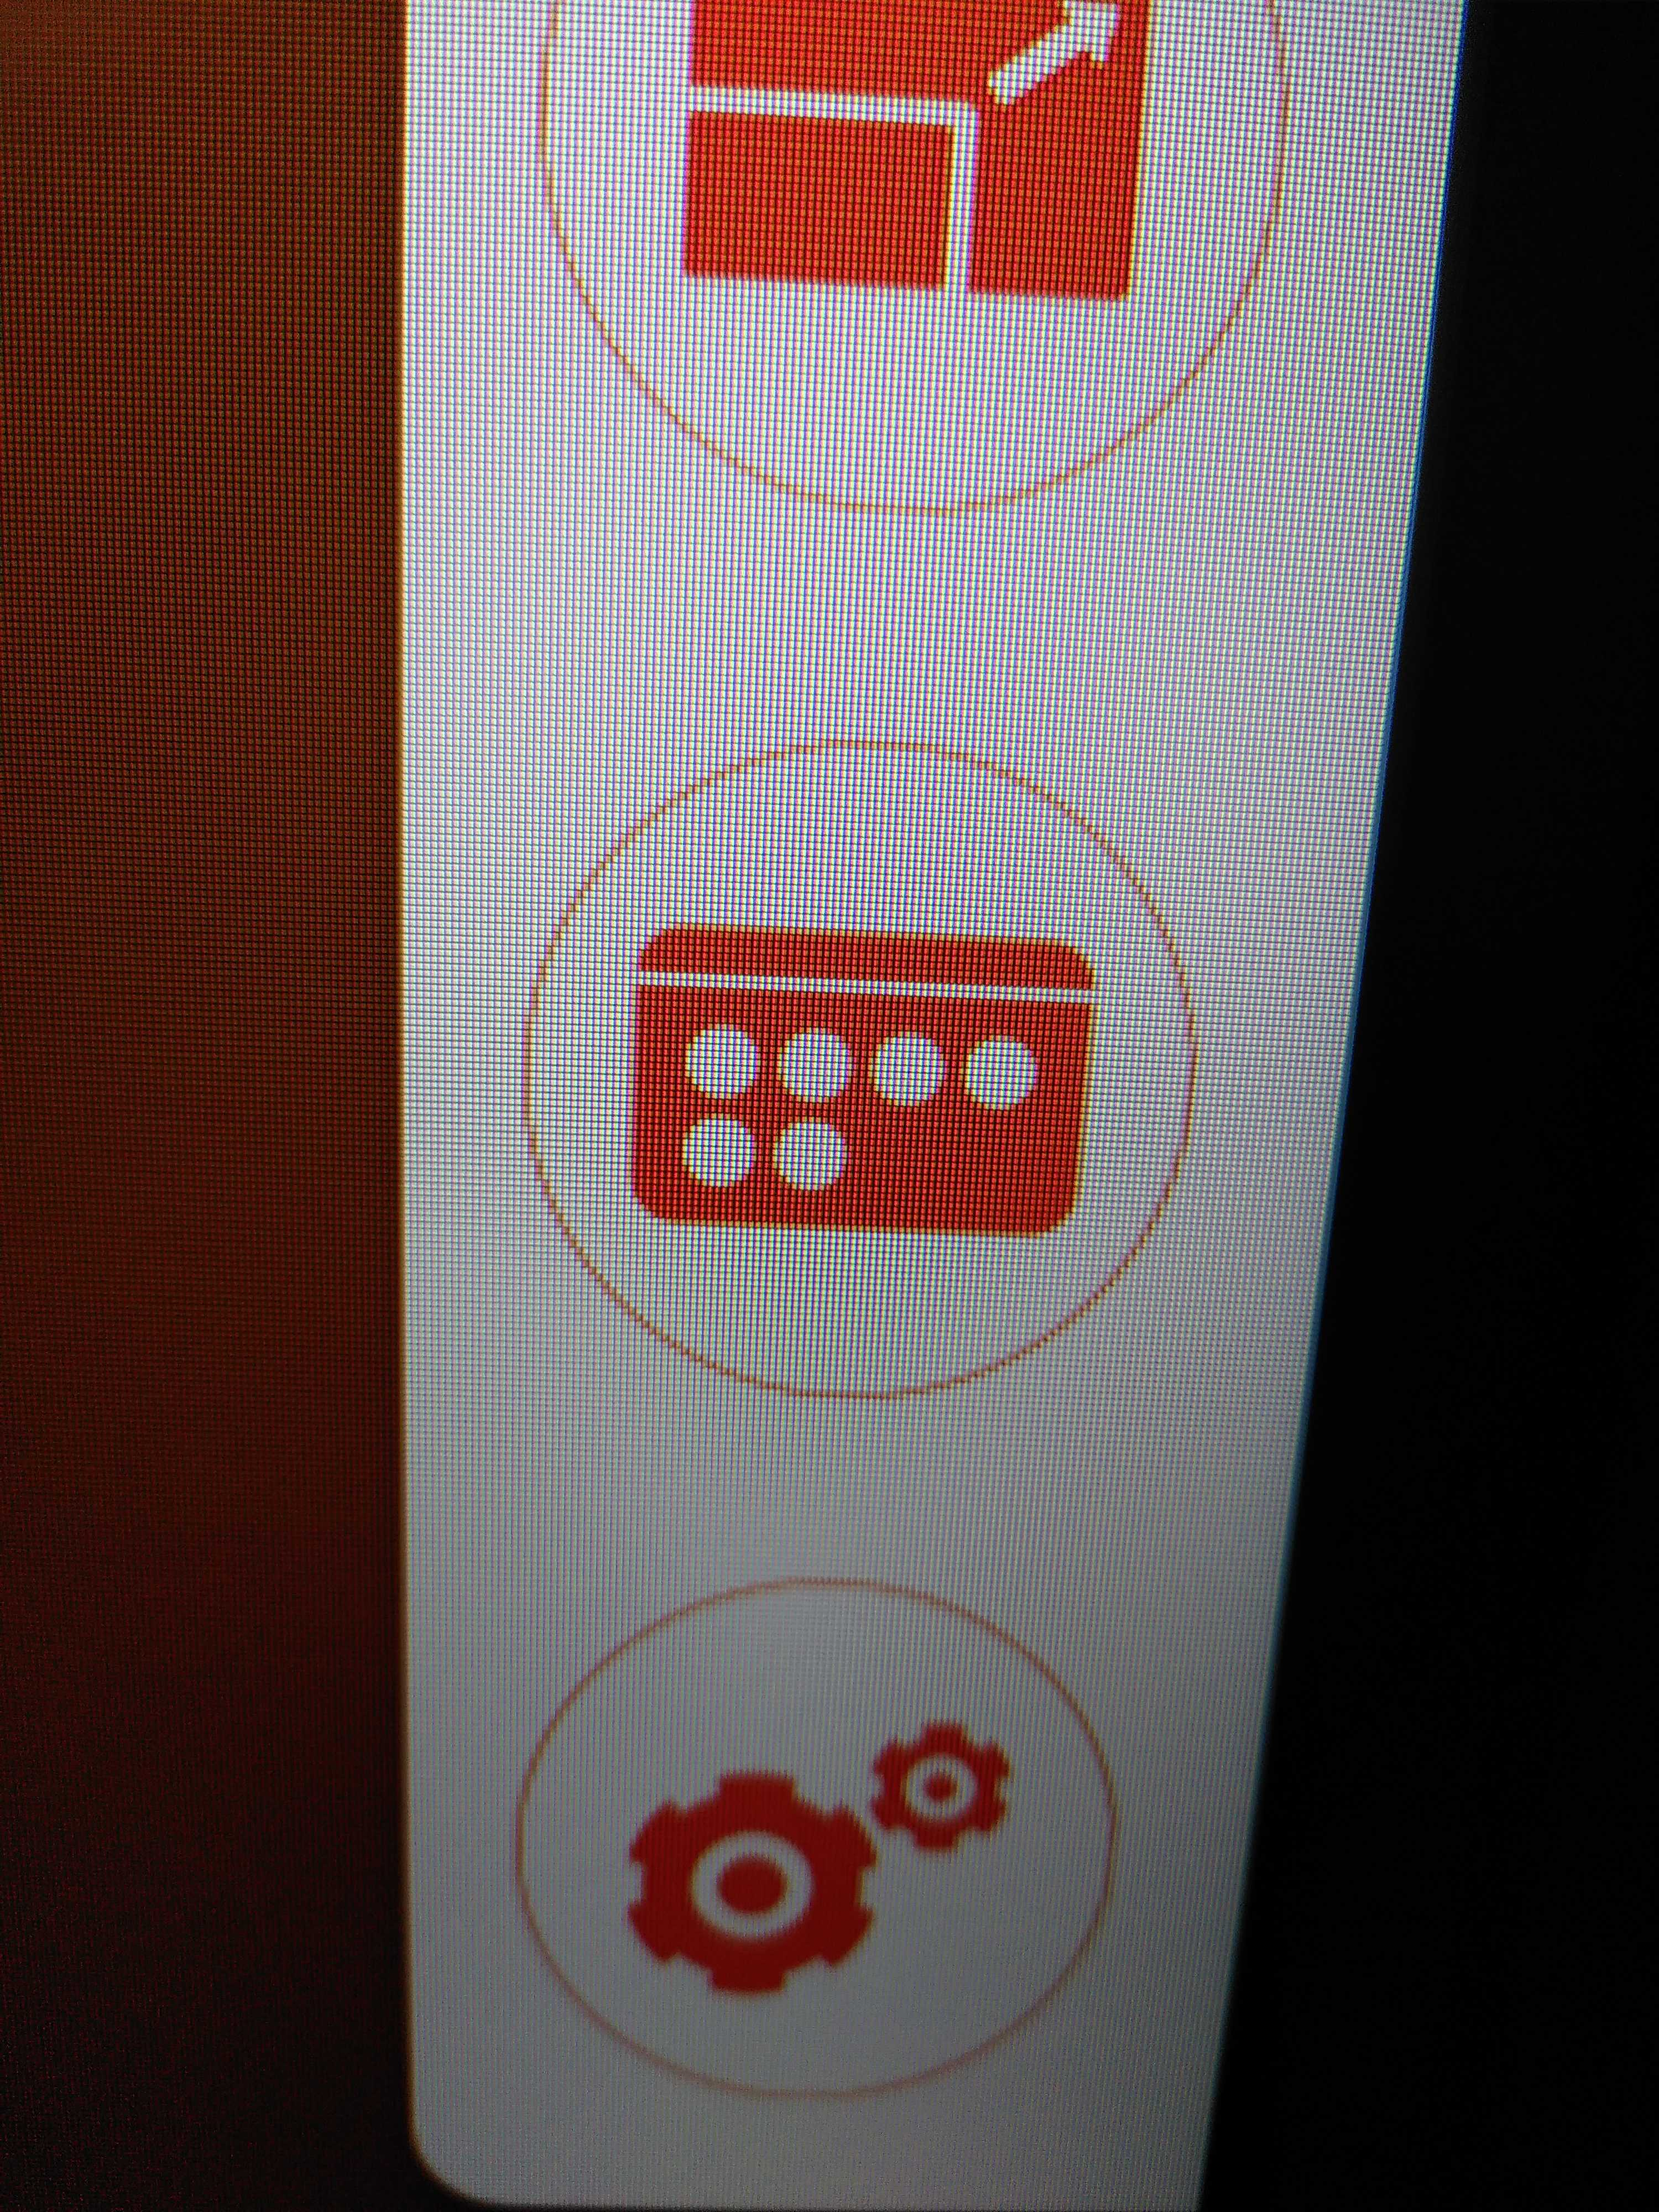
\includegraphics[width=\textwidth]{IMG_20220628_165547.jpg}
		\caption{Symbole "Source"}
		\label{fig:symb-source}
	\end{subfigure}
	\caption{Changement d'interfaces}
\end{figure}


\begin{figure}[h!]
\centering
		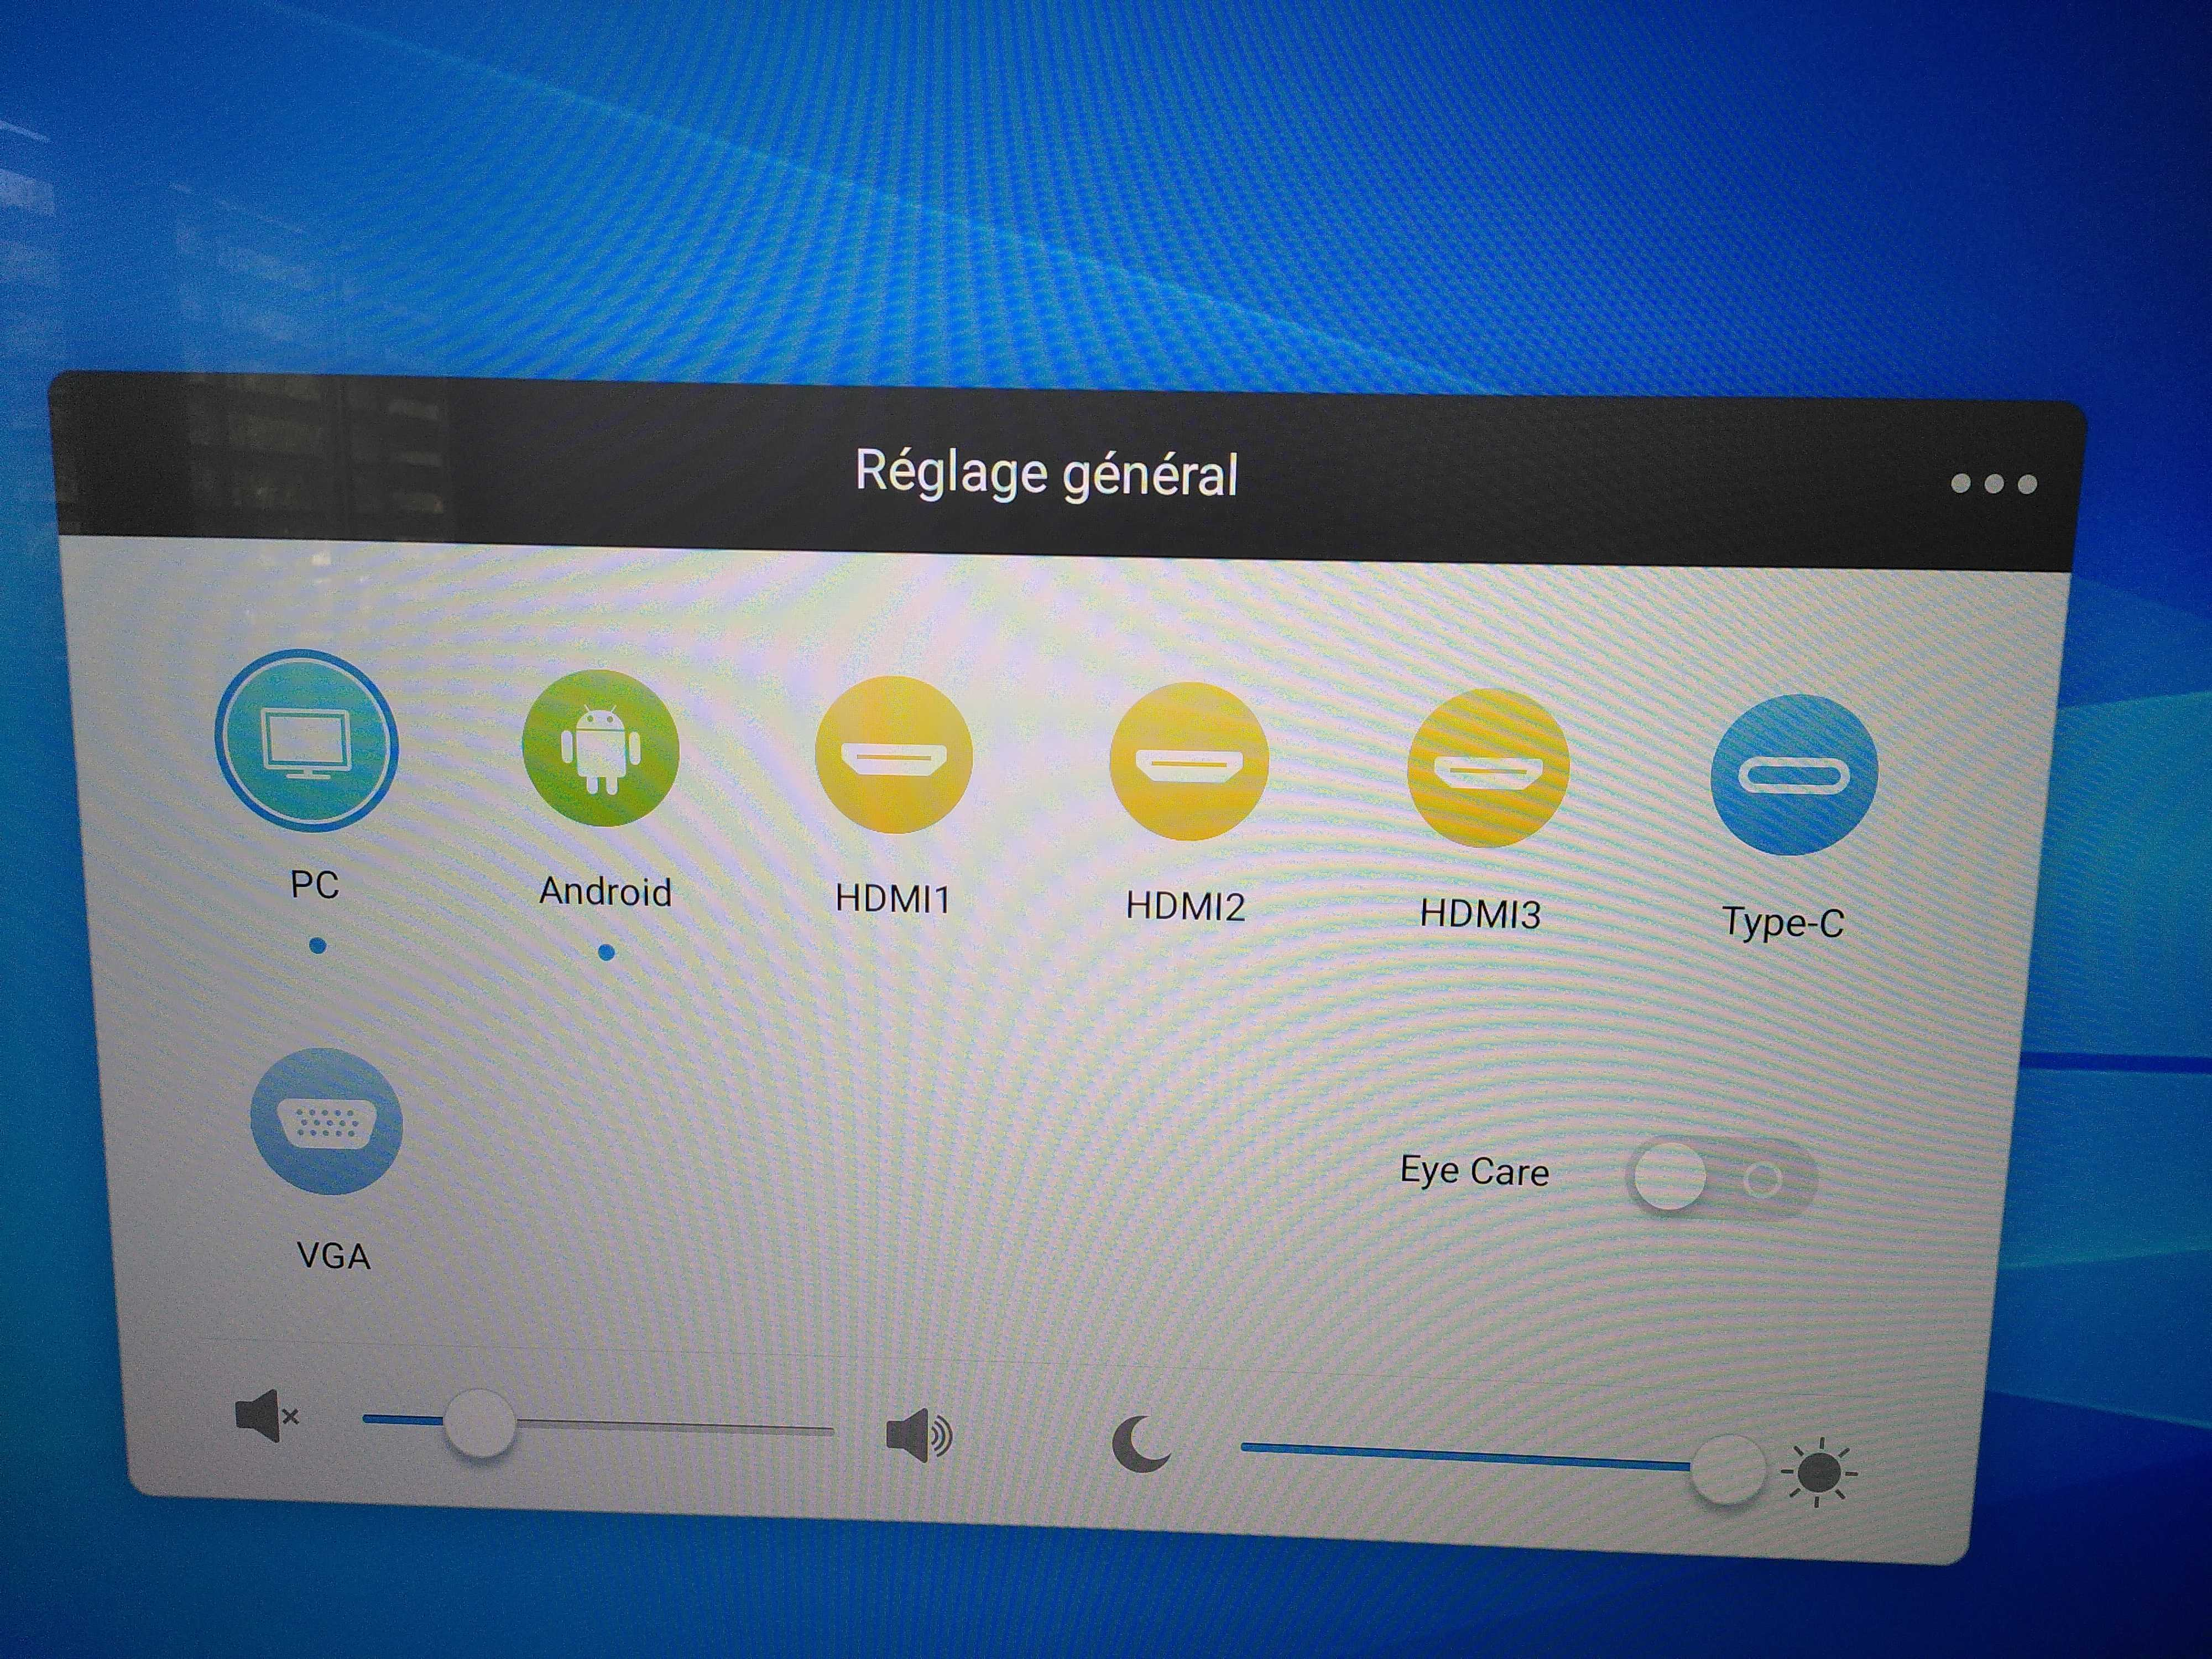
\includegraphics[width=0.7\textwidth]{IMG_20220628_165558.jpg}
		\caption{Symbole "Source"}
		\label{fig:sources}
\end{figure}

%\section{Branchements caméras et autre}
%
%Le branchement de la caméra et autres (cable Ethernet, source HDMI, etc.) dépend du système utilisé.
%Sur le système Windows, les branchements doivent se faire sur la partie supérieure droite de l'écran (au niveau des antennes, Figure \ref{fig:plug-win}). Sous système Android, le branchements se font sur la partie inférieure droite et en dessous de l'écran (Figure \ref{fig:plug-andro}).
% 
%\begin{figure}[h!]
%	\centering
%  	\begin{subfigure}[b]{0.4\textwidth}
%		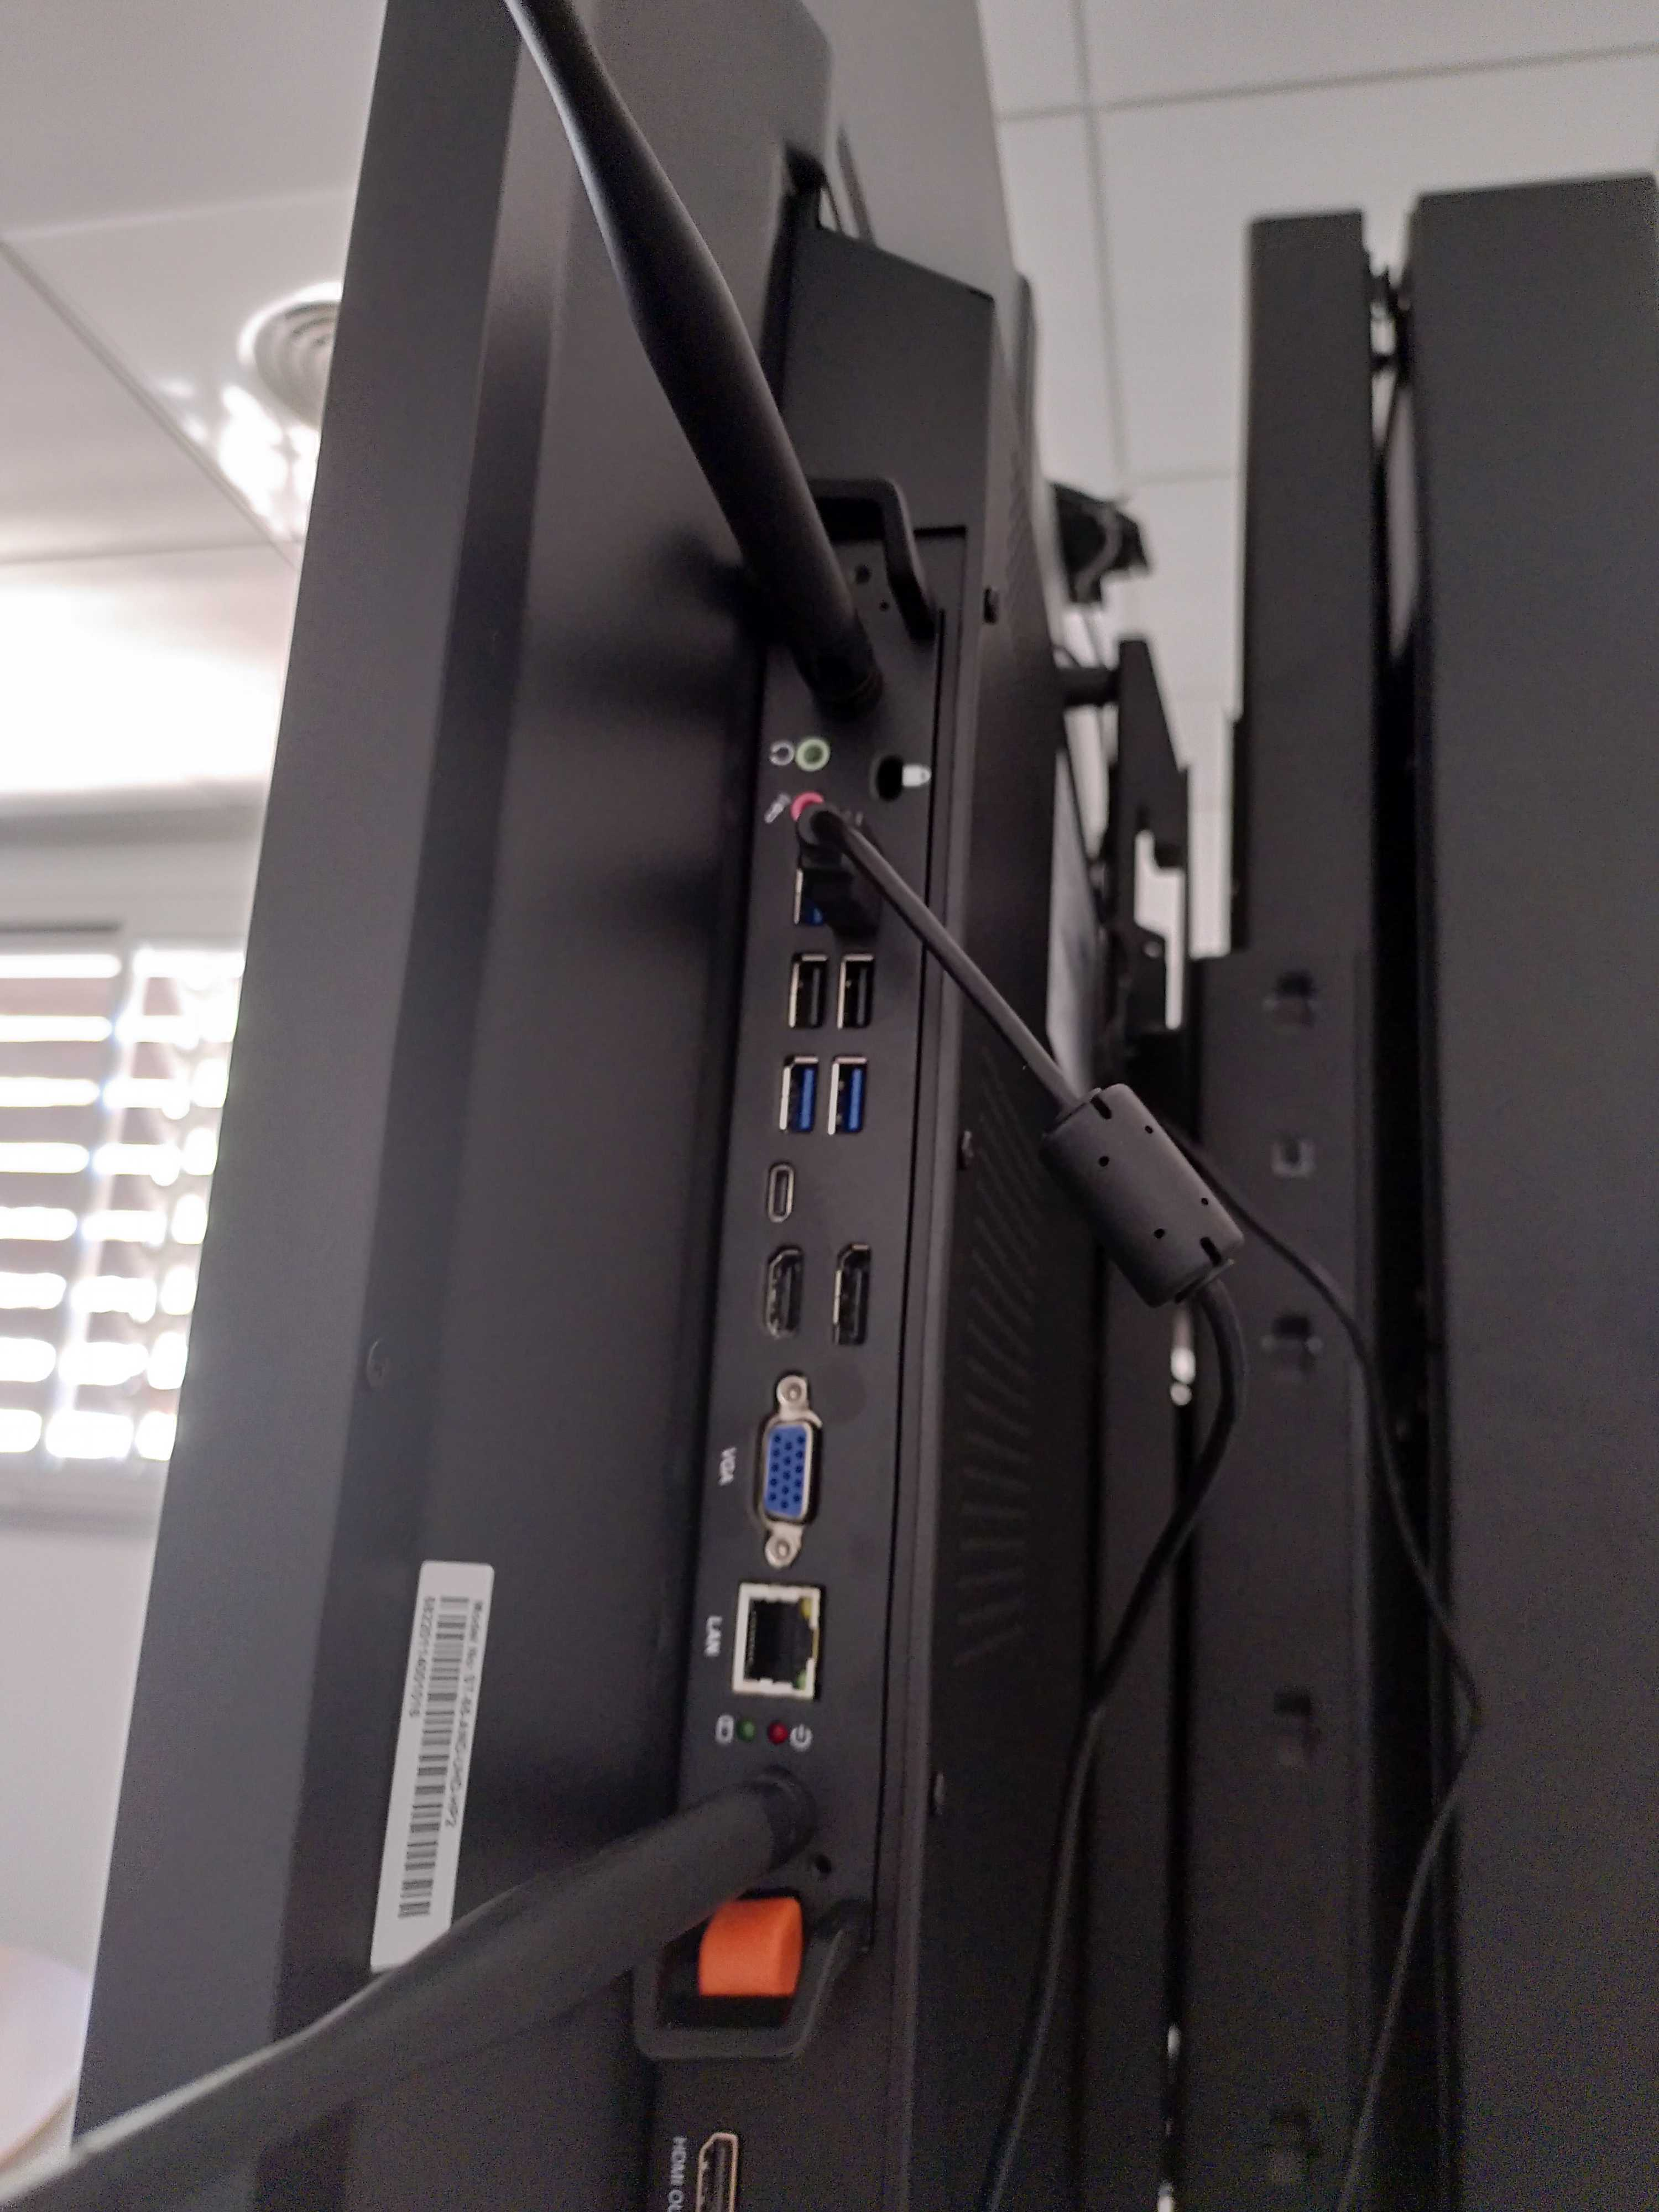
\includegraphics[width=\textwidth]{IMG_20220628_162019.jpg}
%		\caption{Localisation branchements Windows}
%		\label{fig:plug-win}
%	\end{subfigure}
%	\hfill
% 	\begin{subfigure}[b]{0.4\textwidth}
%		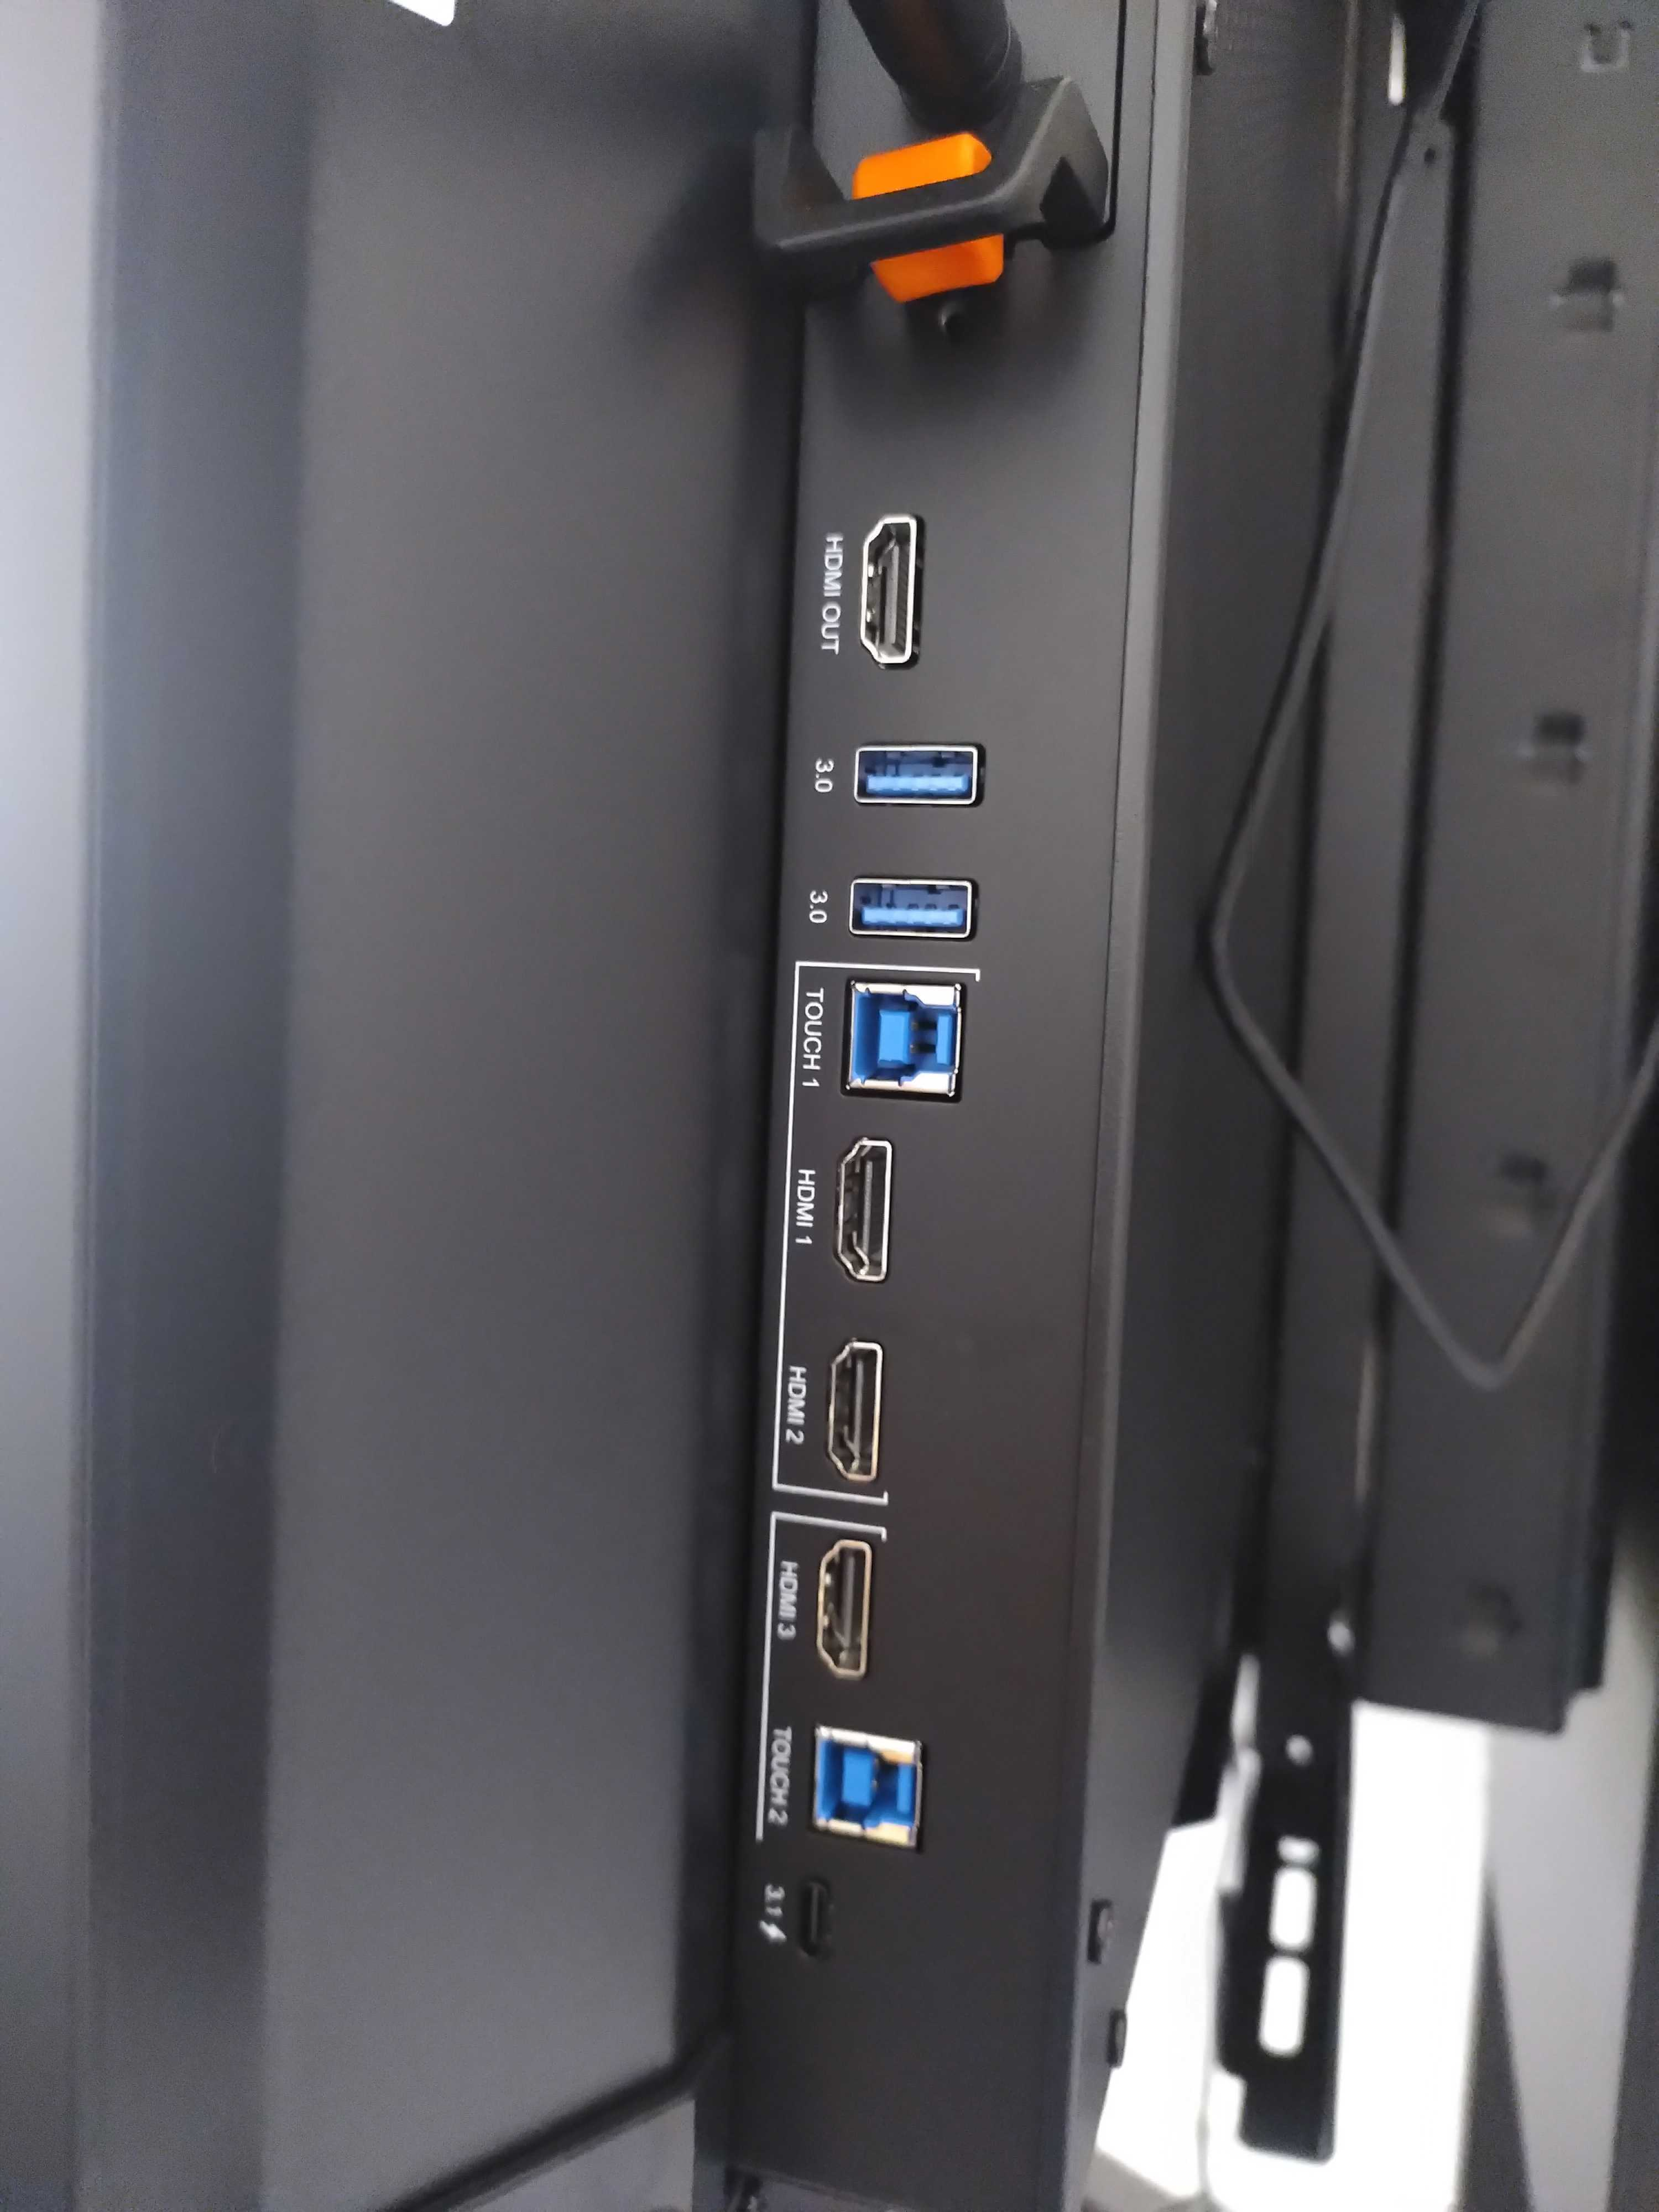
\includegraphics[width=\textwidth]{IMG_20220628_162014.jpg}
%		\caption{Localisation branchements Android}
%		\label{fig:plug-andro}
%	\end{subfigure}
%	\caption{Branchements (camera, etc)}
%\end{figure}

\section{Connection}

\verb+.\Speechitouch+

\section{Zoom}

Les écrans sont associés à une caméra, permettant des visioconférences "petite échelle".\\

Pour lancer Zoom depuis l'interface Windows, cliquer sur le bouton "Démarrer" et rechercher l'application Zoom. \\ 

Pour lancer Zoom depuis l'interface Android, cliquer sur le symbole Applications (en bas au centre de l'ecran, Figure \ref{fig:sys-andro}). Puis choisir Zoom parmi les applications.\\

\end{document}
